Convolutional neural networks can have many different architectures where at least one step of the algorithm features a convolution. 
\subsubsection*{Convolutions}

The mathematical form of a convolution of two functions $f$ and $g$ is given by

\begin{equation}
    (f \ast g)(t) = \int_{-\infty}^{\infty}f(\tau)g(t-\tau)d\tau, 
\end{equation}

which evaluates how the shape of $f$ is modified by $g$. Because image data is only an array of photon counts we can use the discrete convolution

\begin{equation}
    (f \ast g)(t) = \sum_{\tau=-\infty}^{\infty}f(\tau)g(t-\tau).
\end{equation}

In our case, $f$ and $g$ will be tensors. Usually $f$ is called the \textit{input}, $g$ the \textit{kernel} or \textit{filter} and the convolution $(f \ast g)(t)$ the \textit{feature map}. Since our galaxy cluster data is multi-dimensional (see \cref{data_catalogue}), we also have to use a multi-dimensional convolution


\begin{equation}
\begin{split}
    &(f \ast \overset{M}{\cdots} \ast g)(t_1,t_2,\dotsc,t_M) = \\ 
    = \sum_{\tau_1 = - \infty}^{\infty} \sum_{\tau_2 = - \infty}^{\infty} \cdots \sum_{\tau_M = - \infty}^{\infty} &g(\tau_1,\tau_2,\dotsc,\tau_M) f(t_1 - \tau_1, t_2 - \tau_2, \dotsc, t_M-\tau_M).
\end{split}
\end{equation}

For two-dimensional tensors the convolution process can be seen in \autoref{fig:conv_ex}.

\begin{figure}[ht]
 \centering
 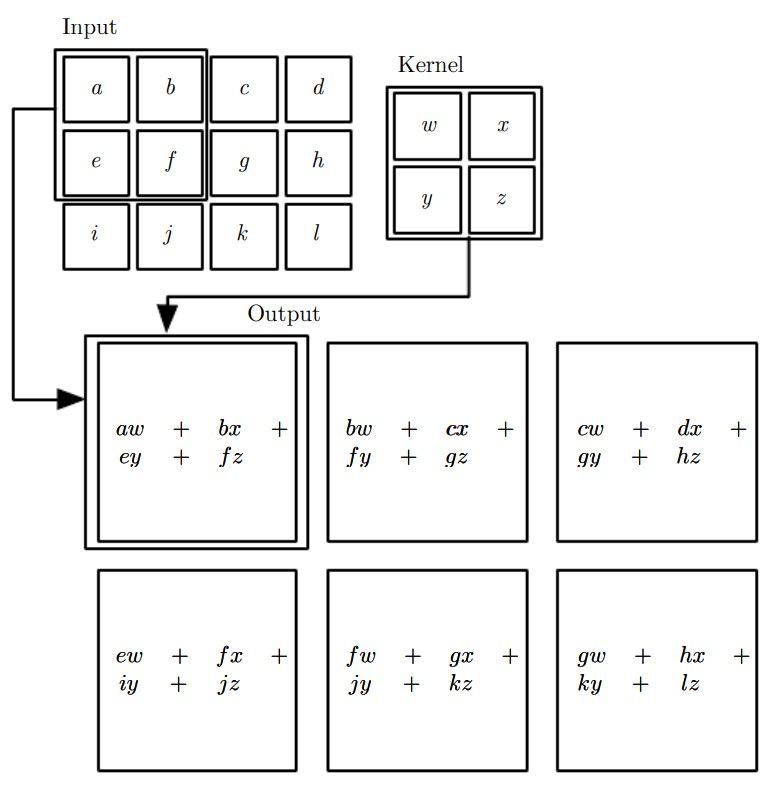
\includegraphics[width=0.66\textwidth]{images/Chapter2/tensor_conv.jpg}
 \caption{Example of a 2D-convolution for an image input with a dimension of 4x3 pixels and a 2x2 kernel resulting in a 3x2 feature map. \citep{Goodfellow-et-al-2016}} 
 \label{fig:conv_ex}
\end{figure}

Training a CNN, we allow the algorithm to evaluate different kernels to help classifying the image. It has been shown that edge detection is one of the most important aspects of image classification. For example the kernel 

\begin{gather}
    g = \begin{bmatrix}
0 & -1 & 0\\
-1 & 4 & -1 \\
0 & -1 & 0
\end{bmatrix}
\end{gather}

is able to highlight edges from input images. To get an idea of how this is executed consider \autoref{fig:seagull}.


\begin{figure}[ht]
 \centering
 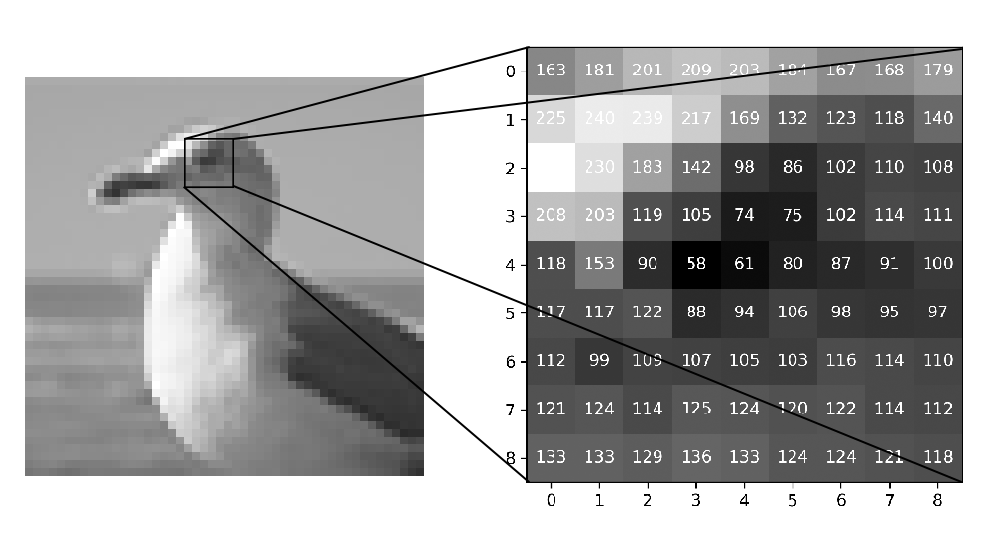
\includegraphics[width=0.66\textwidth]{images/Chapter2/eye_array.png}
 \caption{Image of a seagull in black and white with a size of 50x50 pixels. Every pixel has a value from 1 to 255 indicating its brightness as seen on the right with an extract of 9x9 pixels. By converting this image into a tensor, it is possible to do a two dimensional convolution.} 
 \label{fig:seagull}
\end{figure}
\newpage

Taking only the seagull's eye as input, our tensor has the following shape:

\begin{gather}
    f = \begin{bmatrix}
163 & \cdots & 179\\
\cdots & \cdots & \cdots \\
133 & \cdots & 118
\end{bmatrix}
\end{gather}

Applying the convolution on the whole image we indeed get an outline of the seagull's shape.

\begin{figure}[ht]
 \centering
 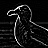
\includegraphics[width=0.4\textwidth]{images/Chapter2/2DConvolved.jpg}
 \caption{Image from \autoref{fig:seagull} after the convolution with the edge outlining kernel $g$.} 
 \label{fig:seagull_conv2d}
\end{figure}

This method indicates why CNNs are so powerful when it comes to image classification. Being able to train and develop filters that can manipulate the input in such a way that it is easier to see patterns, is crucial. \\
Most CNNs are not only build up with convolutions alone. In most cases the combination of one or more convolutions with different mathematical operations helps to increase accuracy. One of these operations is \textit{pooling}.

\subsubsection*{Pooling}
Pooling is another algorithm that helps to simplify the input signal. There are two main pooling operations in machine learning:

\begin{enumerate}
    \item average pooling
    \item max pooling
\end{enumerate}

Although they work in a slightly different manner, they serve the same purpose: helping with translations. If a neural network is supposed to find a certain feature within an image, in most cases it is not necessary to know where the feature is located within the image. Reducing the input to a smaller tensor also helps with training speeds. Average pooling takes the sum over a specific area of the input signal. For example a pooling with a stride of two (see \autoref{fig:pooling}) takes the input of four neighbouring values and reduces them to their average. Max pooling works in a very similar fashion but instead of reducing the neighbouring values to their average, it only keeps the maximum value.

\begin{gather*}
\begin{bmatrix}
\color{green} 50 & \color{blue} 100\\
\color{red} 166 & \color{orange} 24 
\end{bmatrix}
\overset{\text{avg pooling}}{\longleftarrow}
\begin{bmatrix}
\color{green} 163 & \color{green} 17 & \color{blue} 179 & \color{blue} 123\\
\color{green} 0 & \color{green} 21 & \color{blue} 89 & \color{blue} 10 \\
\color{red} 173 & \color{red} 196 & \color{orange} 9 & \color{orange} 15 \\
\color{red} 175 & \color{red} 118 & \color{orange} 62 & \color{orange} 12
\end{bmatrix}
\overset{\text{max pooling}}{\longrightarrow}
\begin{bmatrix}
\color{green} 163 & \color{blue} 179\\
\color{red} 196 & \color{orange} 62 
\end{bmatrix}
\end{gather*}
\captionof{figure}{An input tensor is reduced from 4x4 to 2x2 pixels using average pooling (\textit{left}) and max pooling (\textit{right}) with a stride of two. The colours represent the areas over which the averaging or maximizing takes place.}
\label{fig:pooling}
$\\$
Using these processes with our convoluted image from \autoref{fig:seagull_conv2d}, we can see the effect it has on the input signal.


\begin{figure}[h]
\begin{subfigure}{.5\textwidth}
  \centering
  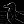
\includegraphics[width=.6\linewidth]{images/Chapter2/avg_pooling.png}
  \caption{Average pooling}
  \label{fig:sfig1}
\end{subfigure}%
\begin{subfigure}{.5\textwidth}
  \centering
  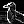
\includegraphics[width=.6\linewidth]{images/Chapter2/max_pooling.png}
  \caption{Max pooling}
  \label{fig:sfig2}
\end{subfigure}
\caption{The different output from pooling of the 48x48 pixel feature map (\autoref{fig:seagull_conv2d}). Both images show less details but preserve the seagull's shape} 
\label{fig:fig}
\end{figure}

While the main features are preserved, the pooling stage reduces complexity and makes training the network more efficient. If we want to do multiple convolutions, we need a way to keep its focus on basic features. As you can see in \autoref{fig:fig}, it is impossible to locate the seagull's eye. But if we just want to know whether we see a seagull or a hummingbird for instance, the exact position of the bird's eye is not that important. This helps to get a higher accuracy and efficiency.
\subsubsection*{Activation Function}
One last missing piece in our CNN block is the activation function. If a CNN block would just consist of convolutions and pooling, it would not be able to find complex features within an input. This is due to the fact that convolutions produce linear activations. This means that the more complex our network gets, we still only have linear connections between the network's layers. While this would work for simple linear regression problems, it is not possible to perform image classification with linearities. To avoid this problem, a non linear function is applied to every block's output. There are a lot of different non linear activation functions with different areas of application. The most simple activation function would be the step function (\autoref{fig:step_f})

\begin{equation}
    f(x) = \begin{cases} \mbox{0} & \mbox{for } x \leq 0 \\ \mbox{1} & \mbox{for } x > 0 \end{cases}.
\end{equation}
Every positive value of the feature map receives the value $1$ while every negative value is changed to $0$. Although this would technically deal with the linearities, it removes most of the details from the input and it would only be useful if we want a binary output. \\

Another option is the hyperbolic tangent function (\autoref{fig:hyptg})

\begin{equation}
    f(x) = \tanh{x} = \frac{e^x - e^{-x}}{e^x + e^{-x}}.
\end{equation}
It can produce values from $-1$ to $1$ and keeps more details than the step function. Activation functions with an output of $-1$ to $1$ or $0$ to $1$ are useful for applications where a possibility should be evaluated.

For more complexity, the rectified linear unit function (ReLU) can be used (\autoref{fig:ReLU})

\begin{equation}
    f(x) = \text{max}(0,x) = \begin{cases}
        \mbox{x} & \mbox{for } x > 0 \\ \mbox{0} & \text{otherwise}
    \end{cases}.
\end{equation}

It leaves positive values unchanged while setting every negative value to zero. It is commonly used in many machine learning approaches because it is very effective in preserving complex details by keeping computing efficiency. Its only downside is the so-called \textit{dying ReLU} problem. If too many activations are set to zero, the neural network is not able to learn anything new. One way to solve this issue is by not setting the negative values to zero, but applying a scaling factor $a$ (usually $0.1$) to them:

\begin{equation}
    f(x) = \begin{cases}
        x & \mbox{for } x > 0 \\ ax & \text{otherwise}
    \end{cases}, \: a = 0.1 \,.
\end{equation}

This is called the Leaky ReLU function (\autoref{fig:L_ReLU}). Despite solving the dying ReLU problem, Leaky ReLU is not always the first choice for machine learning because it also increases computation effort. So it makes sense to first use ReLU and in case of bad predictions switch to other activation functions in optimization.


\begin{figure}[h]
\begin{subfigure}{.5\textwidth}
  \centering
  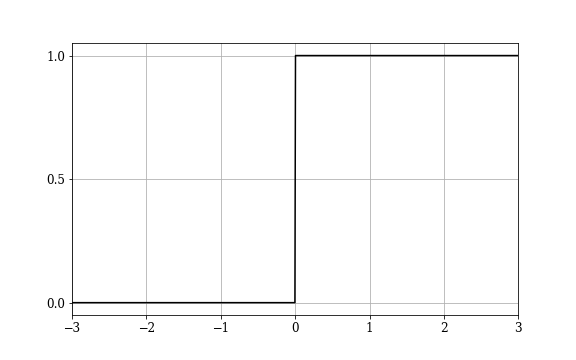
\includegraphics[width=\linewidth]{images/Chapter2/step (1).png}
  \caption{Step function}
  \label{fig:step_f}
\end{subfigure}%
\begin{subfigure}{.5\textwidth}
  \centering
  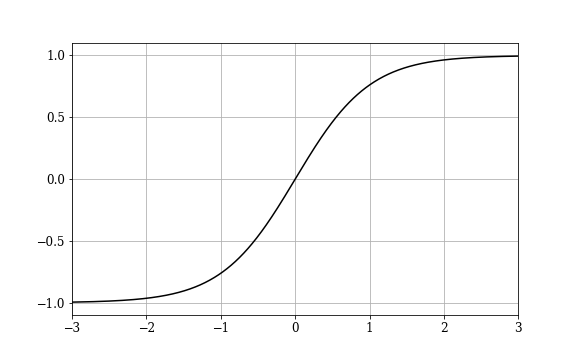
\includegraphics[width=\linewidth]{images/Chapter2/tanh (1).png}
  \caption{Hyperbolic tangent}
  \label{fig:hyptg}
\end{subfigure}
\begin{subfigure}{.5\textwidth}
  \centering
  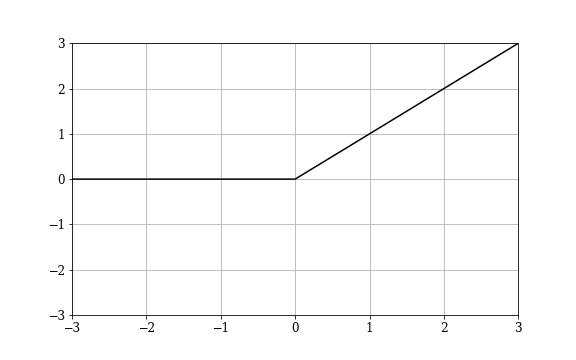
\includegraphics[width=\linewidth]{images/Chapter2/ReLU (1).png}
  \caption{ReLU}
  \label{fig:ReLU}
\end{subfigure}
\begin{subfigure}{.5\textwidth}
  \centering
  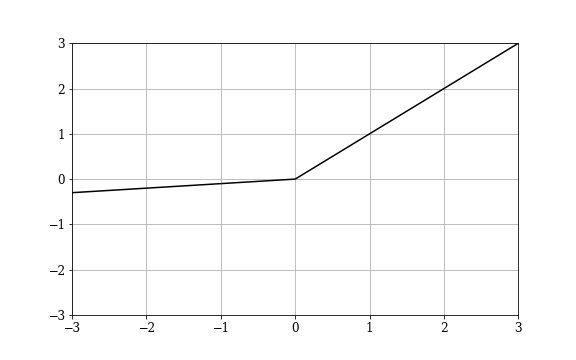
\includegraphics[width=\linewidth]{images/Chapter2/L_ReLU.png}
  \caption{Leaky ReLU ($a=0.1$)}
  \label{fig:L_ReLU}
\end{subfigure}
\caption{Plots of the four different activation functions mentioned} 
\label{fig:activ_functions}
\end{figure}


\subsubsection*{A Basic CNN Block}
Using these three different methods, it is possible to build a simple CNN block (\autoref{fig:CNN_Blocks}). The input tensor is fed into the convolution. Afterwards the feature map is processed via the activation function before applying a pooling. \\
This block can be altered or refined to suit a certain application but you will find this structure in basically every CNN. \citet{Krippendorf_2023} used a slightly altered basic CNN block (\autoref{fig:CNN_Blocks}) consisting of two two-dimensional convolutional layers with ReLU as activation function, average pooling in the first and max pooling in the second layer. 

\newpage

\begin{figure}[h]
\centering
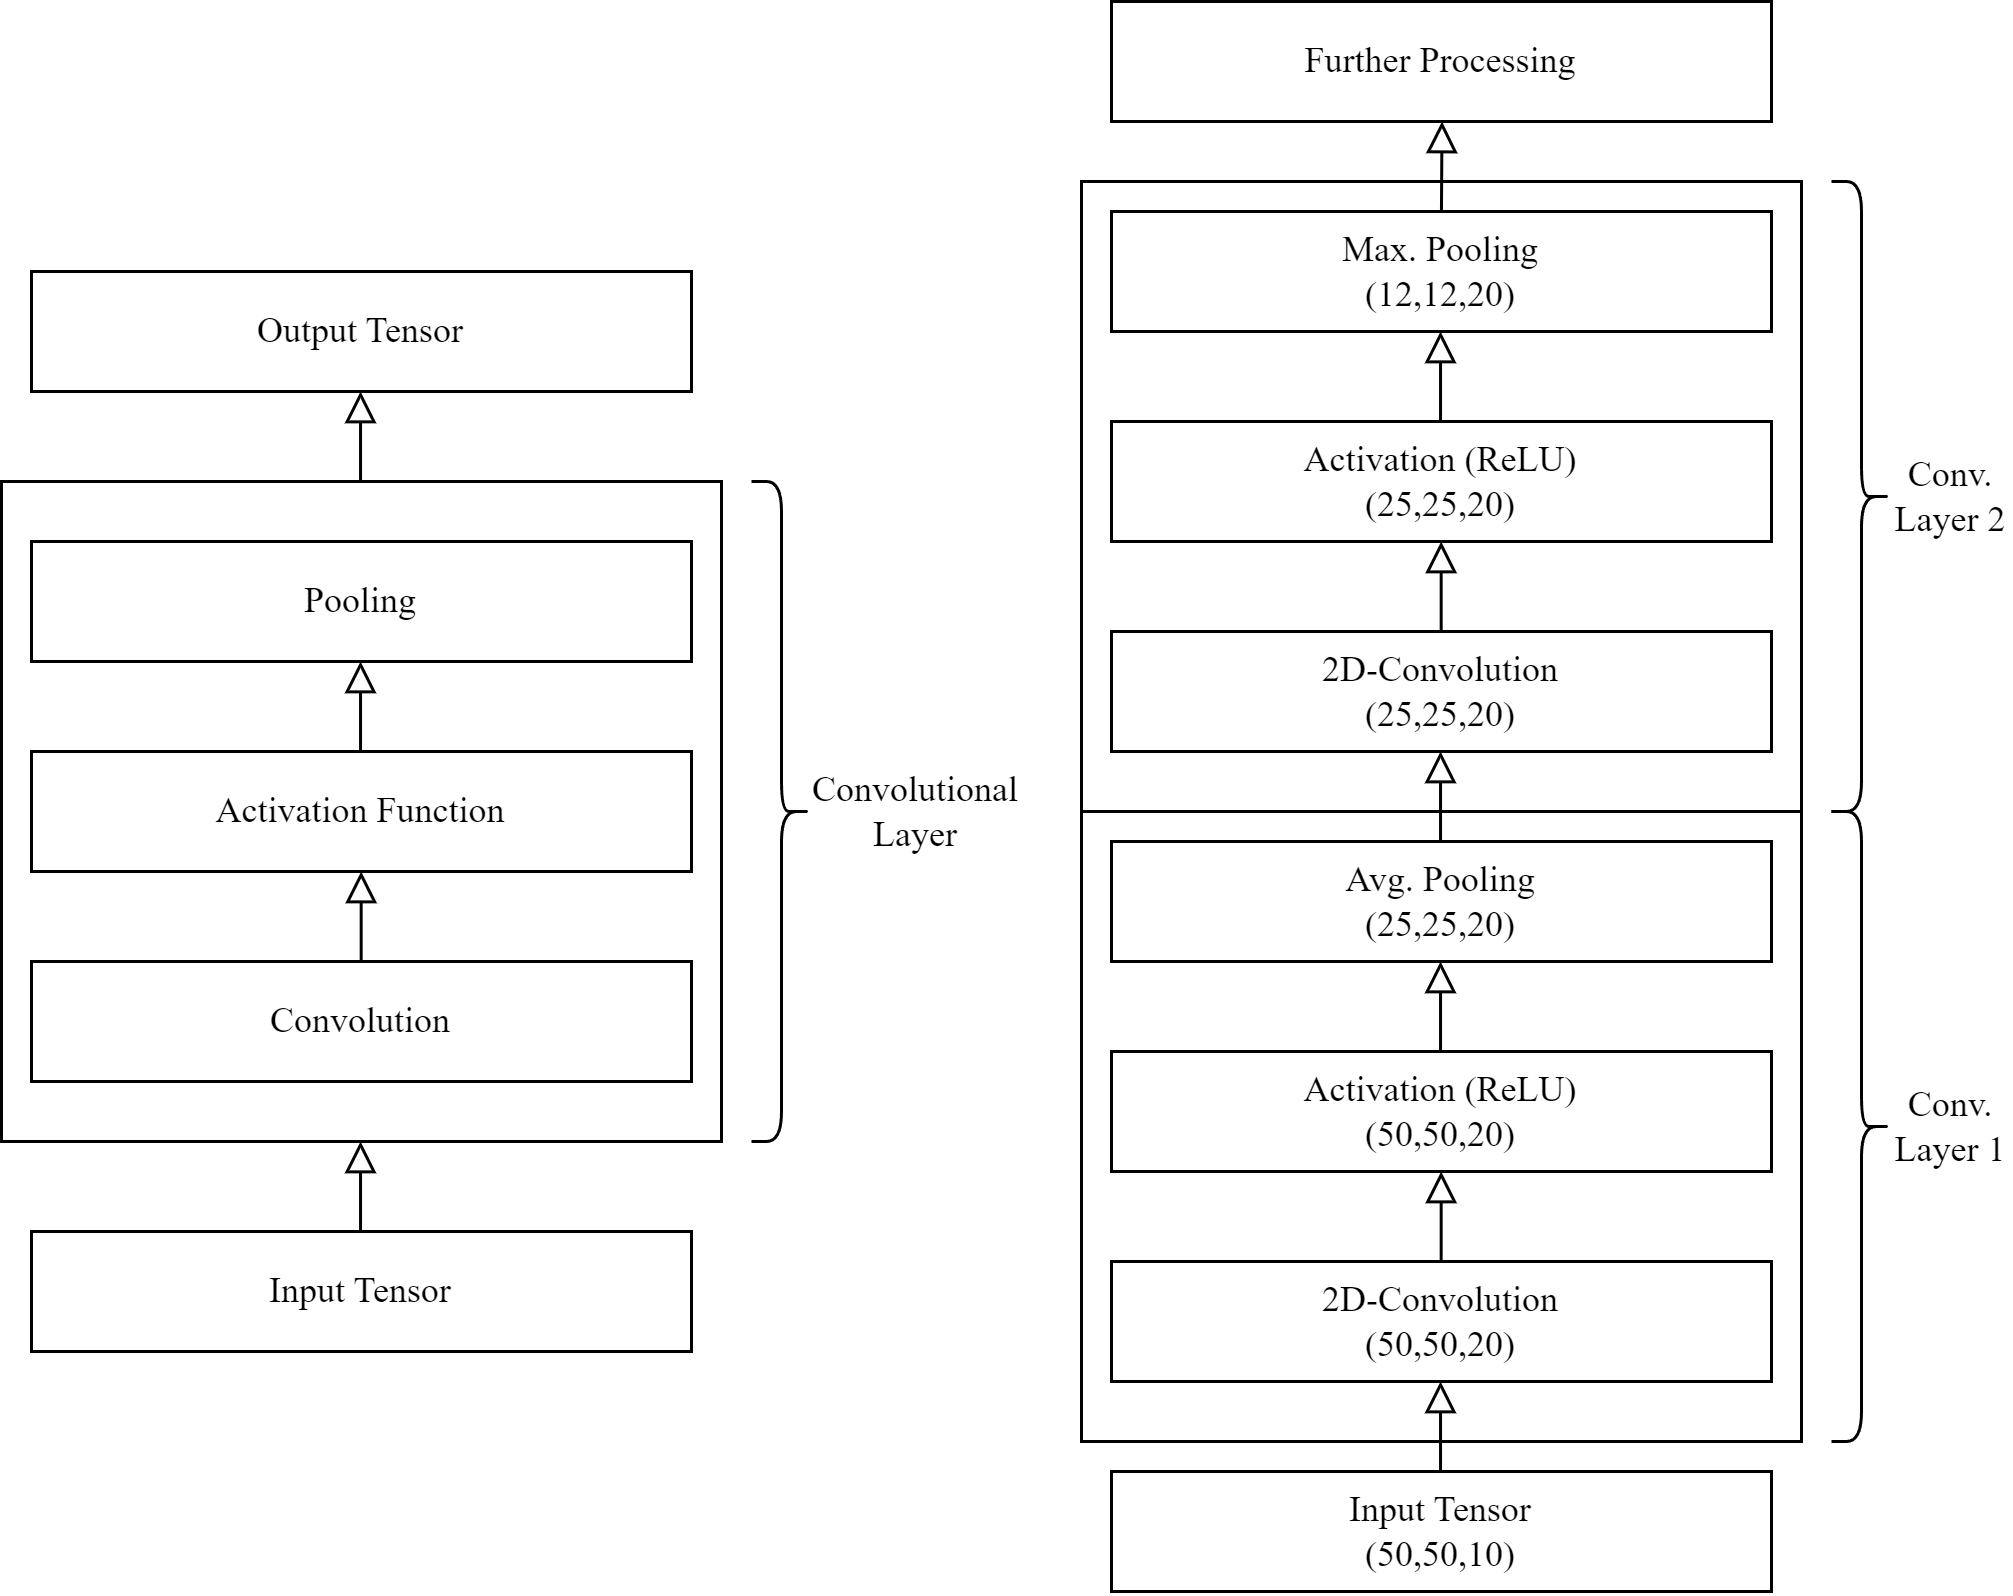
\includegraphics[width=\textwidth]{images/Chapter2/basic_cnn.png}
\caption{Diagrams of a basic CNN structure (\textit{left}) and its application for cluster mass estimation (\textit{right}) (as used in \citealp{Krippendorf_2023}). The convolution, activation and pooling block is referred to as \textit{convolutional layer}. In the application, two convolutional layers are used. The tensor shape is shown below each block.} 
\label{fig:CNN_Blocks}
\end{figure}


In this case, the output tensor of the convolutional layering has a shape of $(12,12,20)$, meaning an array of 12x12 pixels with 20 values for each pixel. However, we only want a single output value since we're interested in the mass of the evaluated galaxy cluster. To achieve this, the output tensor needs to be flattened. This operation puts every pixel and its 20 values into a single vector of the shape $(12\cdot 12 \cdot 20,0,0) = (2880,0,0)$. \\

At this point it is possible to put additional information into the neural network. Consider the \textit{inverse-square law}

\begin{equation}
    I \propto \frac{1}{r^2},
\end{equation}
where $I$ is the intensity of the received light and $r$ is the distance to the light source. This means that without knowing the distance to a light emitting object, it is not possible to estimate the total amount of radiated light. This however is crucial in comparing different galaxy clusters, because a galaxy cluster at a distance of $z=0.6$ can have the same measured intensity as a much bigger galaxy cluster at $z=1.2$.
Providing the neural network with this additional information is as easy as adding it to the vector generated by the flattening, resulting in a shape of $(2881,0,0)$. The next layer after processing the convolutional layer's output is the dense block. This block performs the actual classification of our input. 

\begin{figure}[h]
\centering
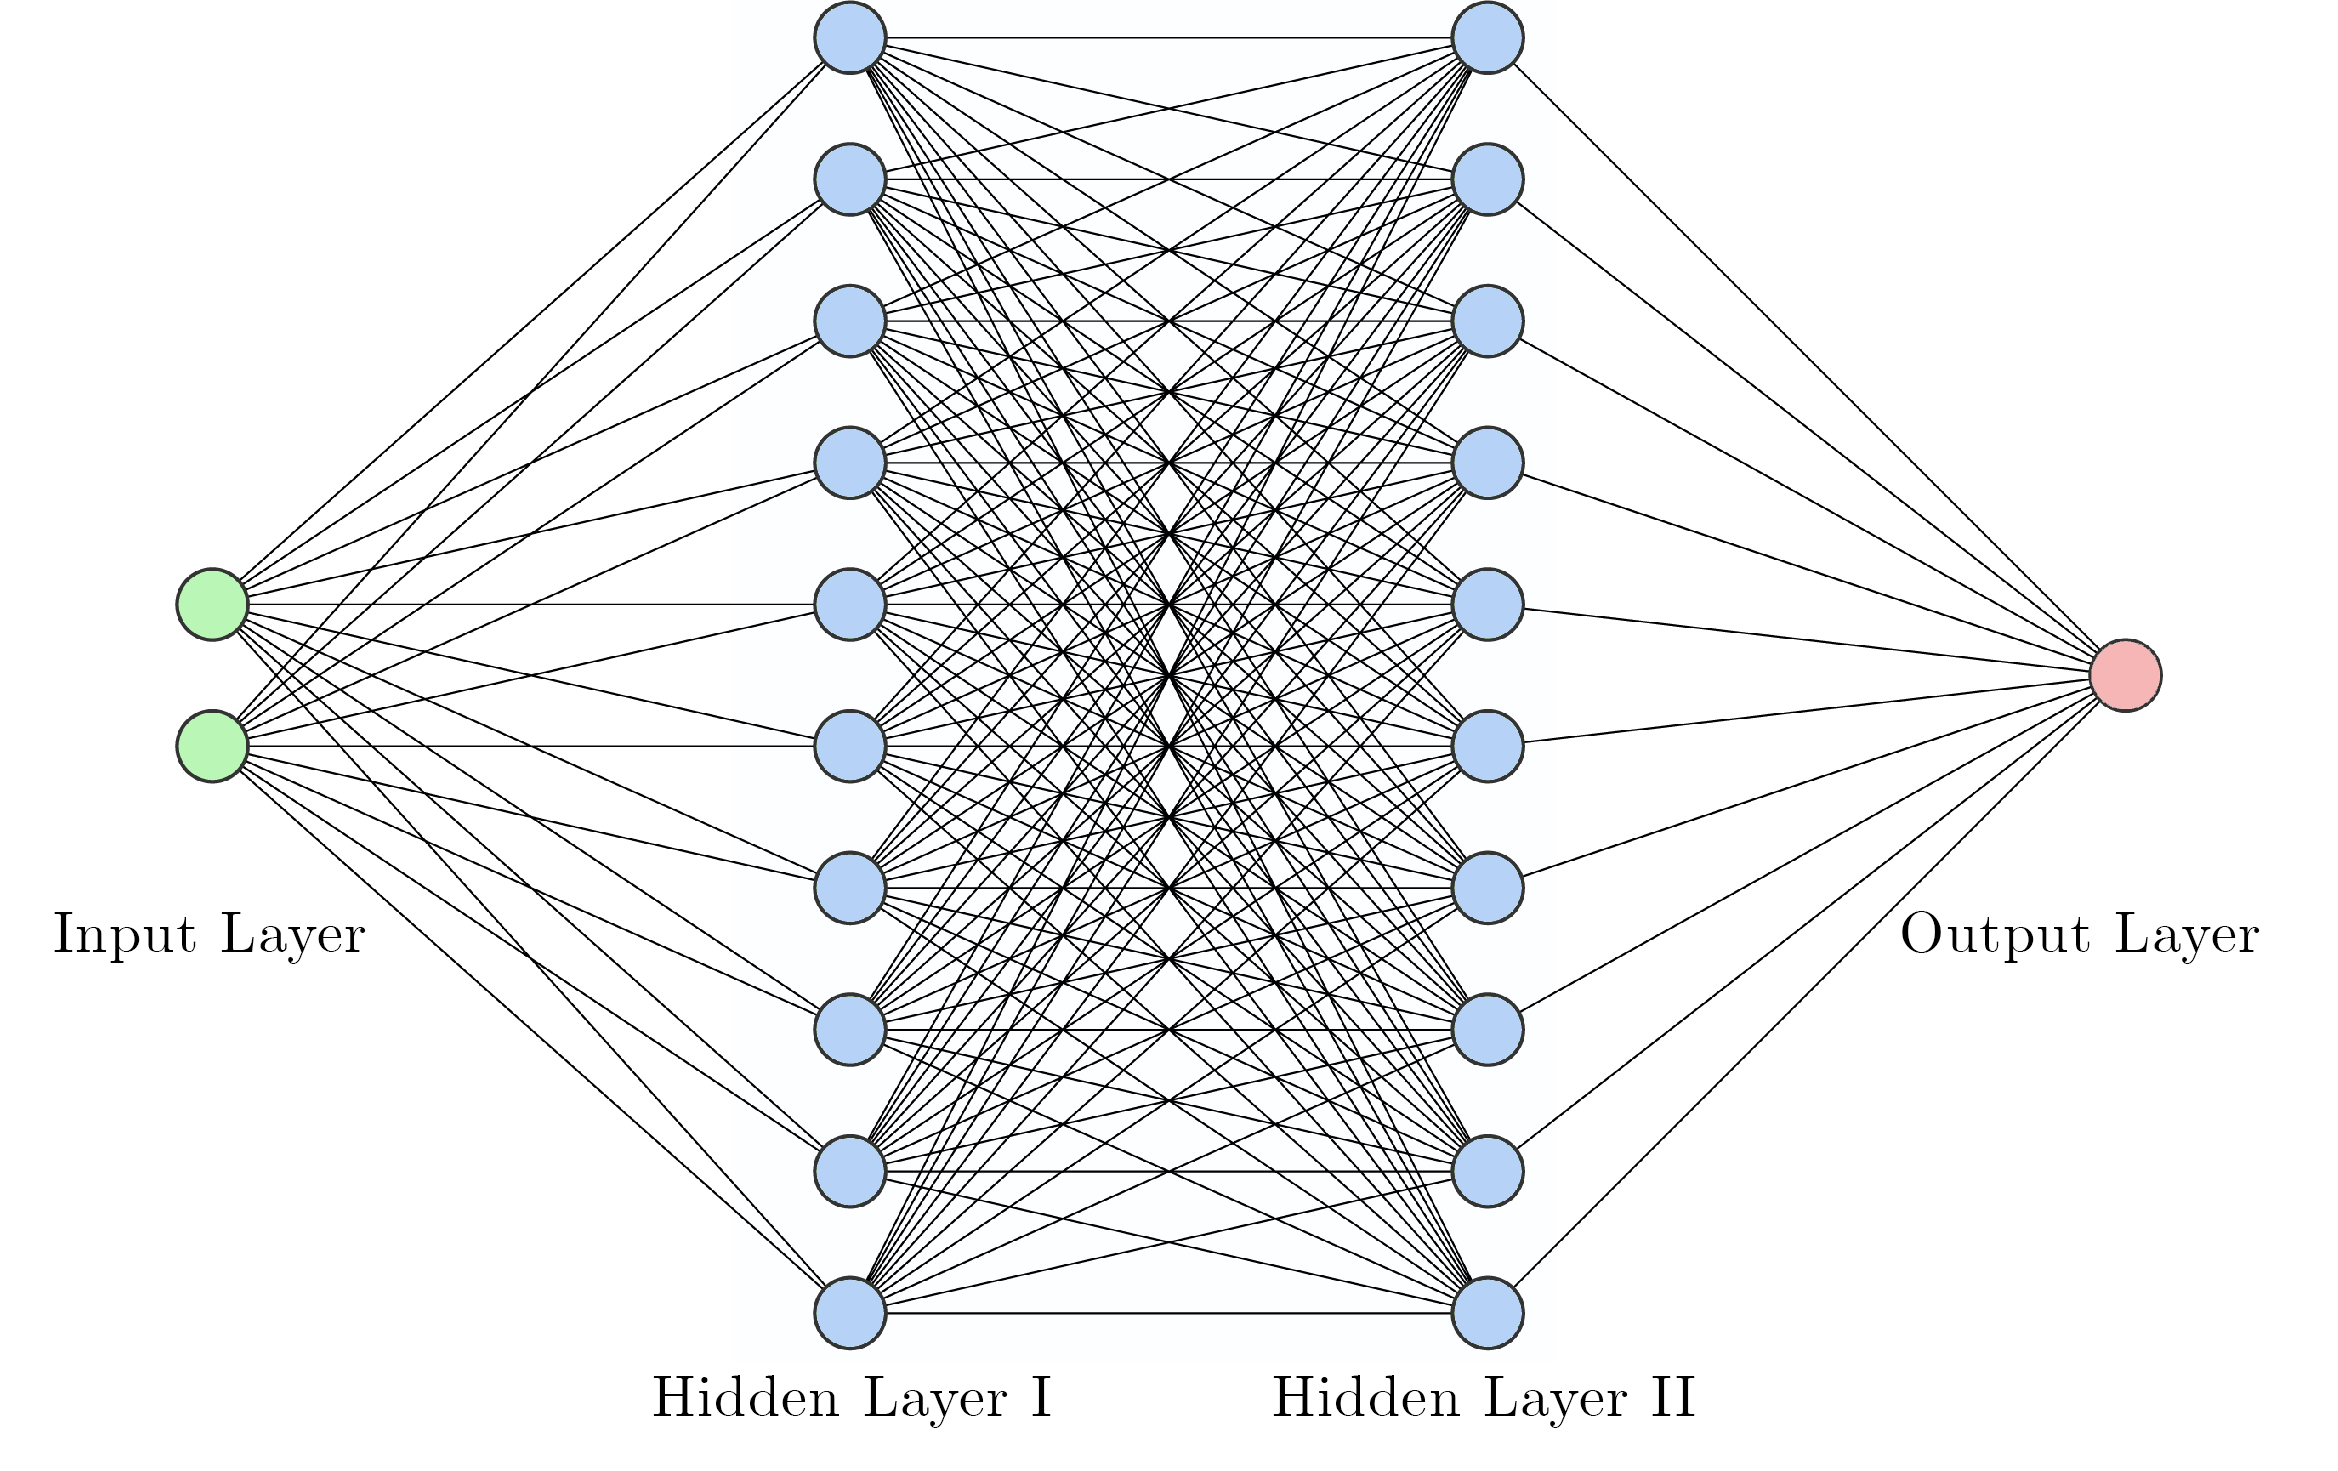
\includegraphics[width=0.9\textwidth]{images/Chapter2/nn.png}
\caption{A dense layer consisting of an input (\textit{green}), two hidden (\textit{blue}) and an output layer (\textit{red}). This can be thought of as the \textit{brain} of every neural network. } 
\label{fig:dense}
\end{figure}

A dense layer, often referred to as \textit{artificial neural network} (ANN) is based on the neuron structure of human and animal brains. It consists of units called \textit{neurons} that are connected to each other to be able to pass on signals. Mathematically, ANNs can be described as the sum of all connections leading to a neuron. For example a neuron $n_i$ receives an input value $x_i$ from a connection to a prior neuron. This specific connection is provided with a \textit{weight} $w_i$ which decides how important the input from this neuron is. Next, the sum over all connections to the neuron and their weights determines the value of this neuron $z$
\begin{equation}
\label{ann}
    z  = \sum \left( (w_1 \cdot x_1) + (w_2 \cdot x_2) + \cdots + (w_n \cdot x_n) \right) = \sum^n_{i=1} w_i \cdot x_i.
\end{equation}
The weights are not the only manipulable parameters. There's also an offset $b$ to the value calculated in \eqref{ann} called \textit{bias}.

\begin{equation}
\label{bias}
    Z  = z + b = \sum^n_{i=1} w_i \cdot x_i + b
\end{equation}
With bias, the algorithm can shift the weighted output in either direction for further evaluation of the importance of specific neurons. Here, another activation function $\Tilde{f}$ is needed in order to archive a certain output. This gives us the final formula for a neuron output with $n$ connections

\begin{equation}
    f(x_i,w_i,b,\Tilde{f}) =  \Tilde{f}(Z) = \Tilde{f} \left( \sum^n_{i=1} w_i \cdot x_i + b \right).
\end{equation}

The activation function is normally provided and tied to the classification task, leaving two trainable parameters, weight and bias.
To know in which direction a machine learning algorithm should alter the weights and biases, it must be provided with a function that needs to be optimised. This is called the \textit{cost} or \textit{loss function}. It provides the neural network with a way of knowing if it gets closer to the real values or not. A commonly used cost function is the \textit{mean squared error} (MSE)

\begin{equation}
\label{MSE}
    L \equiv \text{MSE} = \frac{1}{n}\sum^n_{i=1} \left( X_i - \Tilde{X_i} \right)^2,
\end{equation}

where $n$ is the number of values considered, $X_i$ is the actual given value and $\Tilde{X_i}$ the model's prediction. This function gives the average of the squared errors for a dataset and is used in a variety of machine learning problems. In order to optimise this function, the algorithm performs a \textit{gradient decent}. This means that after changing the weights and the biases, it takes the gradient of the loss function with respect to both parameters

\begin{equation}
    \nabla(L(\Tilde{f},w_i,b)) = \frac{\partial L}{\partial w_i}\hat{w_i}, \frac{\partial L}{\partial b}\hat{b},
\end{equation}
where $\hat{w_i}$ and $\hat{b}$ are unit vectors in the weight and bias space.

The updated parameters are calculated using
\begin{align}
    w_i^{\text{new}} &= w_i - \alpha \cdot \frac{\partial L}{\partial w_i} \; \; \text{and} \\
    b^{\text{new}} &= b - \alpha \cdot \frac{\partial L}{\partial b},
\end{align}

where $\alpha$ is the learning rate. It tells the algorithm how far it is allowed to go towards the gradient. Especially with overfitting problems, the learning rate must be chosen carefully. If an algorithm is learning too quickly, it can find a minimum in the loss function that might be a good fit for the input data but does not work with data is has not seen during training. We will address this issue in \cref{train_params}.\\

Finally we have a complete and trainable neural network (see \autoref{fig:final_network}) with multiple convolutional layers. 

\begin{figure}[H]
\centering
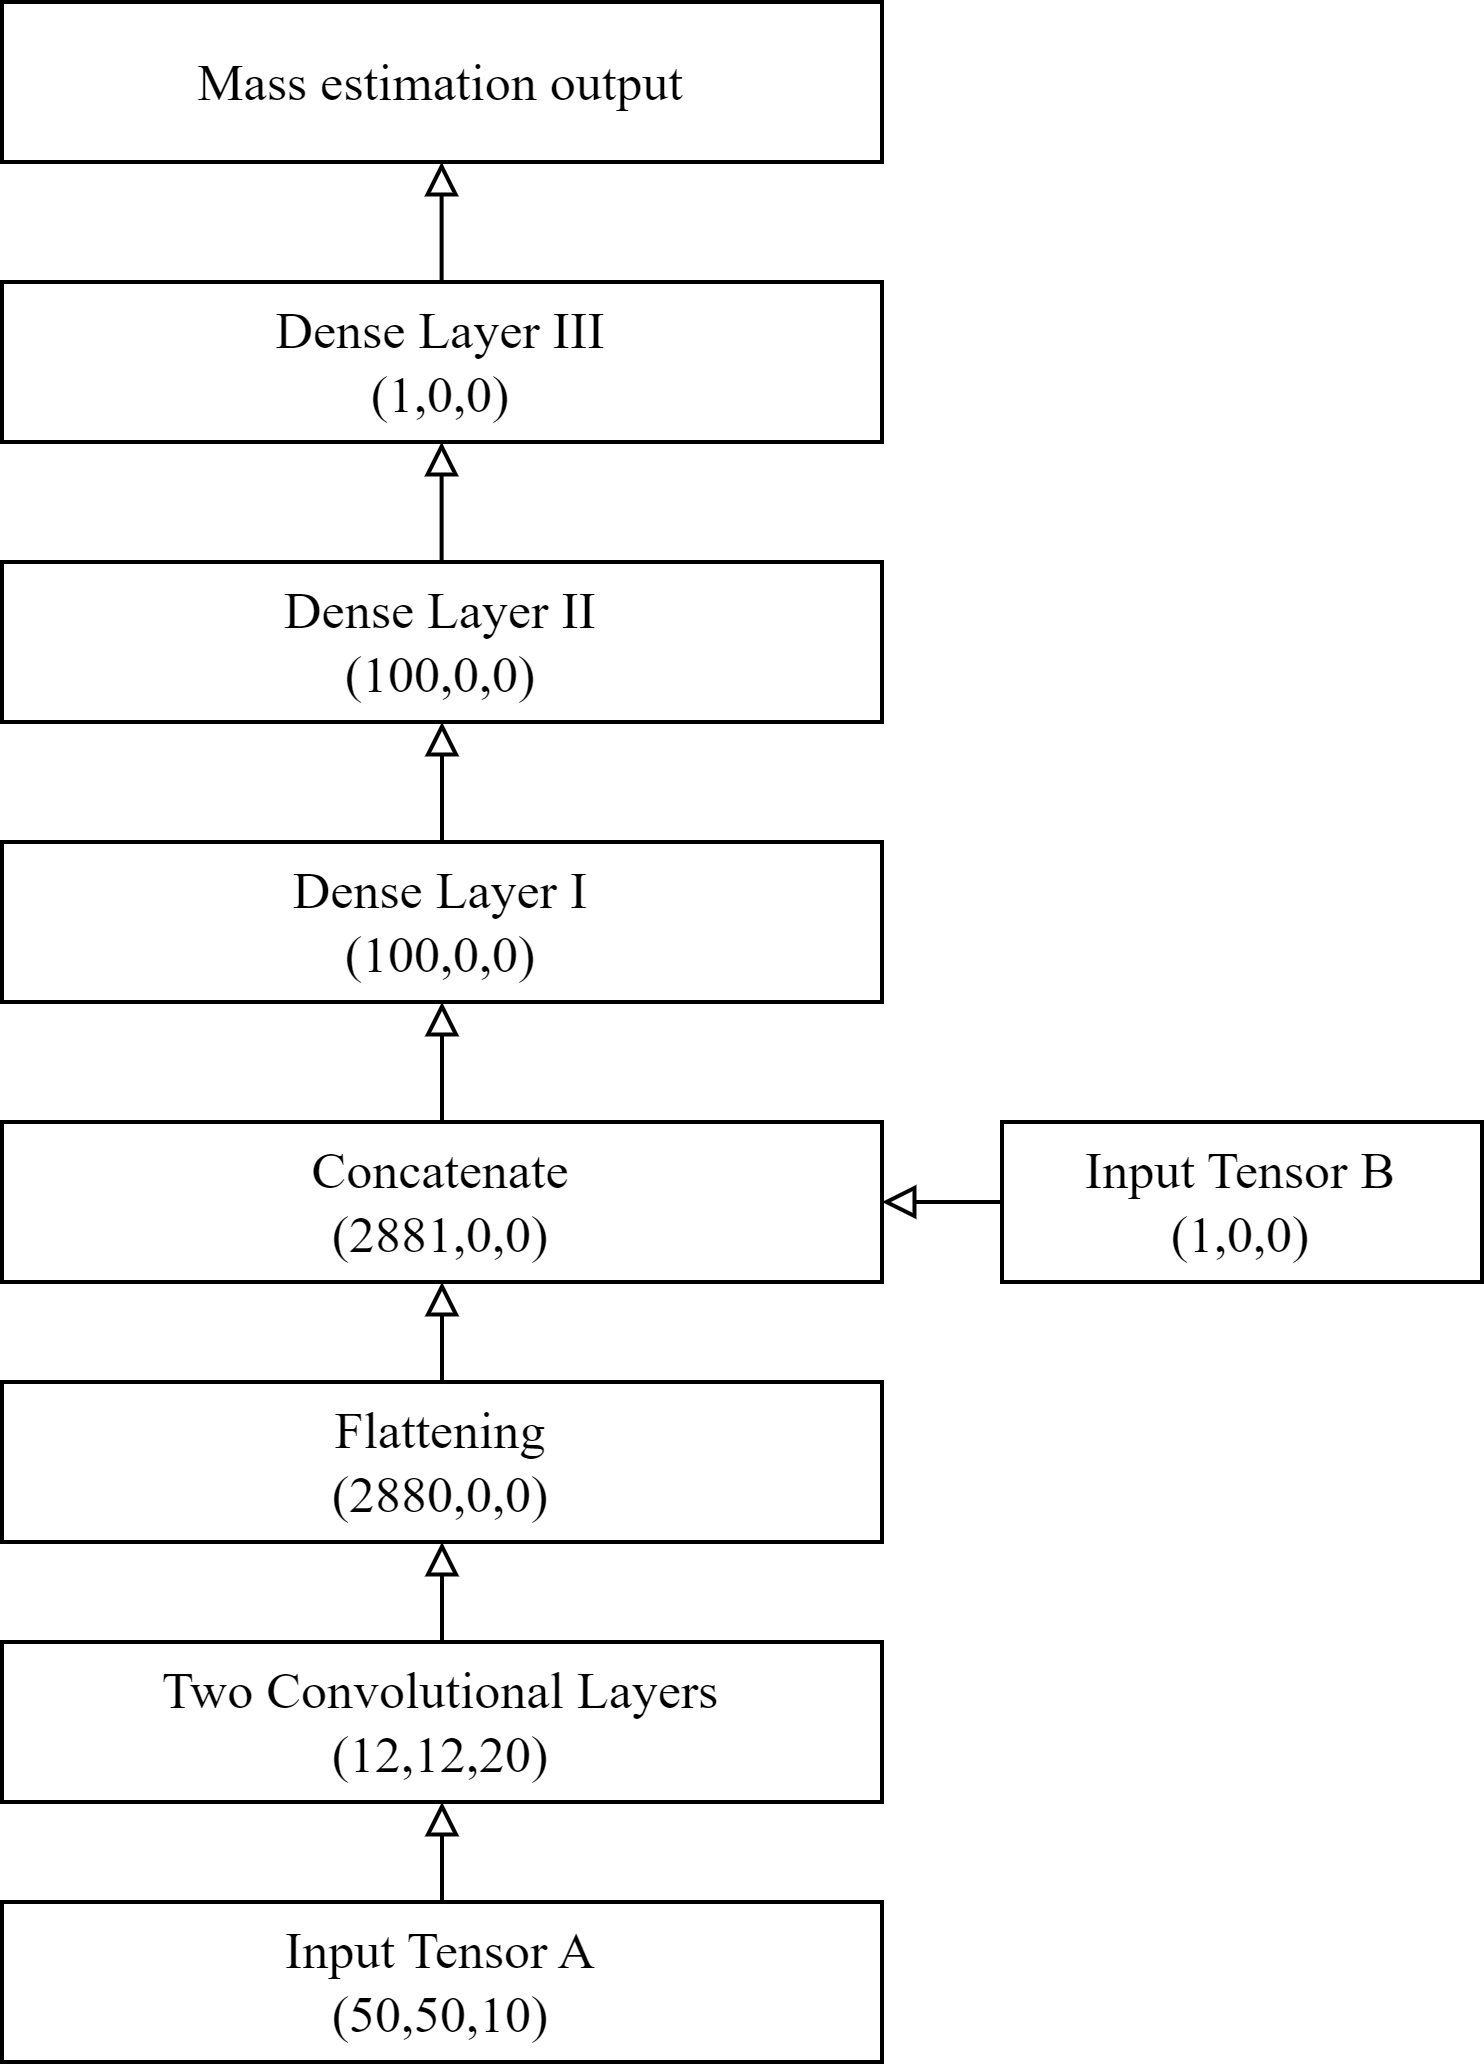
\includegraphics[width=0.4\textwidth]{images/Chapter2/basic.png}
\caption{The final processing of our convoluted input from \autoref{fig:CNN_Blocks}. The output tensor shape is shown below the block labeling. Input A is the input of the X-ray images and input B is the input of the redshift data.} 
\label{fig:final_network}
\end{figure}










